\documentclass{article}
\usepackage{graphicx} % Required for inserting images
\graphicspath{{./images/}}
\usepackage[utf8]{inputenc}
\usepackage{amsthm}
\usepackage{amsmath}
\usepackage{amssymb}
\usepackage{mathtools}
\usepackage[hidelinks]{hyperref}
\usepackage[a4paper]{geometry}

\title{%
    Caractérisation des singularités de type $\J$ \\ [2ex]
    \large Stage de recherche de premier cycle sous la supervision de \\
    Frédéric Rochon et Carlo Scarpa}
\author{Félix Larose-Gervais}
\date{Été 2023}

\newtheorem{definition}{Définition}
\newtheorem{proposition}{Proposition}
\newtheorem{conjecture}{Conjecture}
\newtheorem{example}{Exemple}
\newtheorem{corollary}{Corollaire}
\renewcommand*{\proofname}{Preuve}

\newcommand{\J}{\mathfrak{J}}
\newcommand{\JS}{\overline{\J}}
\renewcommand{\contentsname}{Table des matières}

\begin{document}

\maketitle

\tableofcontents

\newpage

\section{Introduction}

\subsection{Motivation}

Ce document tire sa source des travaux\cite{apostolov2016ale} de Vestislav Apostolov et Yann Rollin, 
et tente d'étudier les singularités de type $\J$ en adoptant un point de vue algébrique.
On y répond a une question ouverte, énonce quelques propriétés du type $\J$, et commence à caractériser 
une version plus stricte notée $\JS$.

\subsection{Notations}

Soient $a, b \in \mathbb{Z}$. On note la relation de coprimalité $\perp$

\[ a \perp b \iff \gcd(a, b) = 1 \]
Soient $m, n \in \mathbb{N}$, $X$ un ensemble. Notons 

\begin{itemize}
    \item $S_m$ le groupe symétrique à $m$ lettres;
    \item $\mathbb{Z}_n$ l'anneau des entiers modulo n ($\mathbb{Z}/n\mathbb{Z}$);
    \item $\mathbb{Z}_n^\times$ son groupe d'inversibles ($\{ a \in \mathbb{Z}_n \mid a \perp n \})$;
    \item $X^m$ l'ensemble des m-tuplets de $X$ $(\underbrace{X \times \cdots \times X}_{m fois})$.
\end{itemize}
On notera aussi $S_n^m$ l'ensemble des m-tuplets d'inversibles modulo n $({({\mathbb{Z}_n^\times})}^m)$.

\subsection{Définitions}

\begin{definition}
    Une \textbf{singularité} est un m-tuplets $[a] = ([a_1], \dots, [a_m]) \in S_n^m$. On appelle \begin{itemize}
        \item $n$ la \textbf{racine} de la singularité;
        \item $[a_1], \dots, [a_m]$ les \textbf{poids} de la singularité.
    \end{itemize}
\end{definition}

\begin{definition}
    Un \textbf{éclatement} $a \in \mathbb{Z}^m$ d'une singularité $[a] \in S_n^m$ (noté $a \in [a]$) est un choix de 
    représentant $a = (a_1, \dots, a_m)$ tel que
    \begin{align*}
        \forall i \neq j & : a_i \perp a_j.
    \end{align*}
    On note $E_a$ l'ensemble des singularités associées à l'éclatement $a$ comme suit:
    \begin{align*}
        E_a & = \{ [a^i] \in S_{a_i}^m \mid \forall i = 1..m,\; a_i > 1 \} \text{ où}\\
        [a^i] & = ([a^i_1], \dots, [a^i_m]) \in S_{a_i}^m \text{ avec} \\
        [a^i_j] & \equiv \begin{cases}
            -n & \text{si $i = j$} \\
            a_j & \text{sinon}
        \end{cases} \pmod{a_i} \quad \forall j = 1..m
    \end{align*}
    On appelle $a = (a_1, \dots, a_m)$ \textbf{l'éclatement naturel} de $[a]$ si 
    les $a_1, \dots, a_m$ sont les plus petits représentants positifs de leurs classes.
\end{definition}

\begin{definition}
    Un éclatement $a \in [a]$ est dit \textbf{lisse} si $a = (1, \dots, 1)$.
\end{definition}

\begin{definition}
    En procédant récursivement, on dit qu'une singularité $[a]$ est de \textbf{type $\J$} (noté $[a] \in \J$)
    si $[a]$ possède un éclatement lisse ou s'il existe $a \in [a]$ tel que $E_a \subset \J$.

    De même, en procédant récursivement, on dit qu'une singularité $[a]$ est de \textbf{type $\J$ strict} (noté $[a] \in \JS$) lorsque 
    pour $a \in [a]$ l'éclatement naturel de $[a]$ on a que $a$ est lisse ou que $E_a \subset \JS$.
\end{definition}

\newpage

\subsection{Arbre d'éclatements}

Calculer l'arbre d'éclatements d'une singularité permet de la classifier 
comme de type $\J$ ou non. Il est obtenu en appliquant récursivement la définition 2
et en vérifiant les coprimalités nécessaires à chaque étape.

\begin{figure}[h]
    \caption{Arbre d'éclatement montrant ${(7, 3)}_{10} \in \JS$}
    \centering
    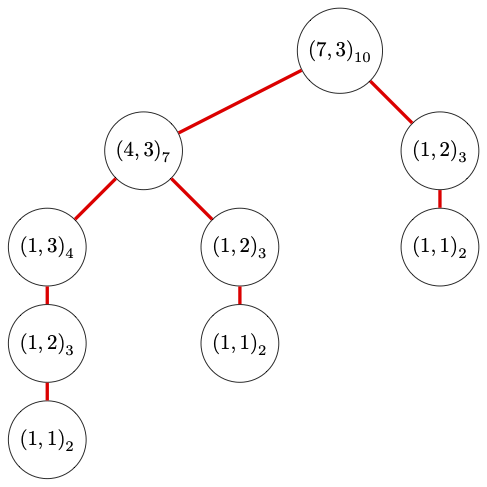
\includegraphics[width=0.55\textwidth]{10_7_3}
\end{figure}

On remarque dans l'exemple suivant que les noeuds ${(2, 2)}_3$ et ${(3, 3)}_4$ ne 
respectent pas les coprimalités nécessaires et donc ne sont pas de type $\JS$.
La singularité racine de l'arbre ${(5, 3)}_{16}$ n'est donc pas de type $\JS$.

\begin{figure}[h]
    \caption{Arbre d'éclatement montrant ${(5, 3)}_{16} \not \in \JS$}
    \centering
    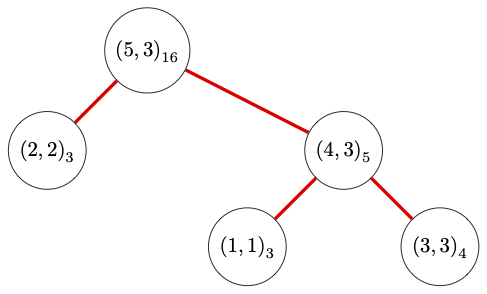
\includegraphics[width=0.55\textwidth]{16_5_3}
\end{figure}

\newpage

\subsection{Rappels d'arithmétique}

\subsubsection{Algorithme d'Euclide et plus grand diviseur commun (PGDC)}

Soient $a, b \in \mathbb{Z}$. On peut calculer le plus grand diviseur commun $\gcd(a, b)$ de $a$ et $b$ en procédant récursivement comme suit (supposant $\gcd(a, b) > 0$):
\begin{align*}
    \gcd(a, b) & := \begin{cases}
        a & \text{ si $b = 0$,} \\
        \gcd(b, a \mod b) & \text{ sinon.}
    \end{cases}
\end{align*}
Avec $k \in \mathbb{Z}$, on a les propriétés suivantes:
\begin{align*}
    \gcd(a, 1) & = 1, \\
    \gcd(a, b) & = \gcd(b, a), \\
    \gcd(a, b) &= \gcd(a, -b), \\
    \gcd(a, b) & = \gcd(a, b + ka).
\end{align*}
De la dernière on déduit directement, pour $n \in \mathbb{N}$, que
\begin{align*}
        a \equiv b \pmod n \implies \gcd(a, n) = \gcd(b, n).
\end{align*}

\subsubsection{Théorème des restes chinois}

Soient $m, n_1, \dots, n_m \in \mathbb{N}$ et $a_1, \dots, a_m \in \mathbb{Z}$. Notons le produit $n = n_1 \cdots n_m$.

Si $\forall i \neq j : n_i \perp n_j$, alors $\exists!x \in \mathbb{Z}_n$ tel que
\begin{align*}
    x &\equiv a_1 \pmod {n_1}, \\
    &\vdotswithin{\equiv} \\
    x &\equiv a_m \pmod {n_m}.
\end{align*}

Cette solution, pour $m = 2$,
\begin{align*}
    x \equiv a_1 \pmod {n_1} \\
    x \equiv a_2 \pmod {n_2}
\end{align*}

est obtenue comme suit:

Puisque $n_1 \perp n_2$, on a $s, t \in \mathbb{Z}$ tels que $1 = sn_1 + tn_2$

Et donc $x = a_1tn_2 + a_2sn_1$ est l'unique solution $\pmod {n_1n_2}$

Cette méthode nous laisse $m - 1$ équations dans le système

Ainsi, pour $m > 2$, il suffit d'itérer le processus jusqu'à ce qu'il n'en reste qu'une.

\newpage

\subsection{Résultats connus}
Résultats utiles, dus à Habib Jaber\cite{jaber2022stage}.

\begin{proposition}
    Si $a, b \in \mathbb{Z}$, alors
    \[ a \perp b \implies {(a, b)}_{a + b} \in \JS. \]
\end{proposition}

\begin{example}
    $8 \perp 5 \implies {(8, 5)}_{13} \in \JS$
\end{example}
\begin{figure}[h]
    \caption{Illustration avec la suite de Fibonacci}
    \centering
    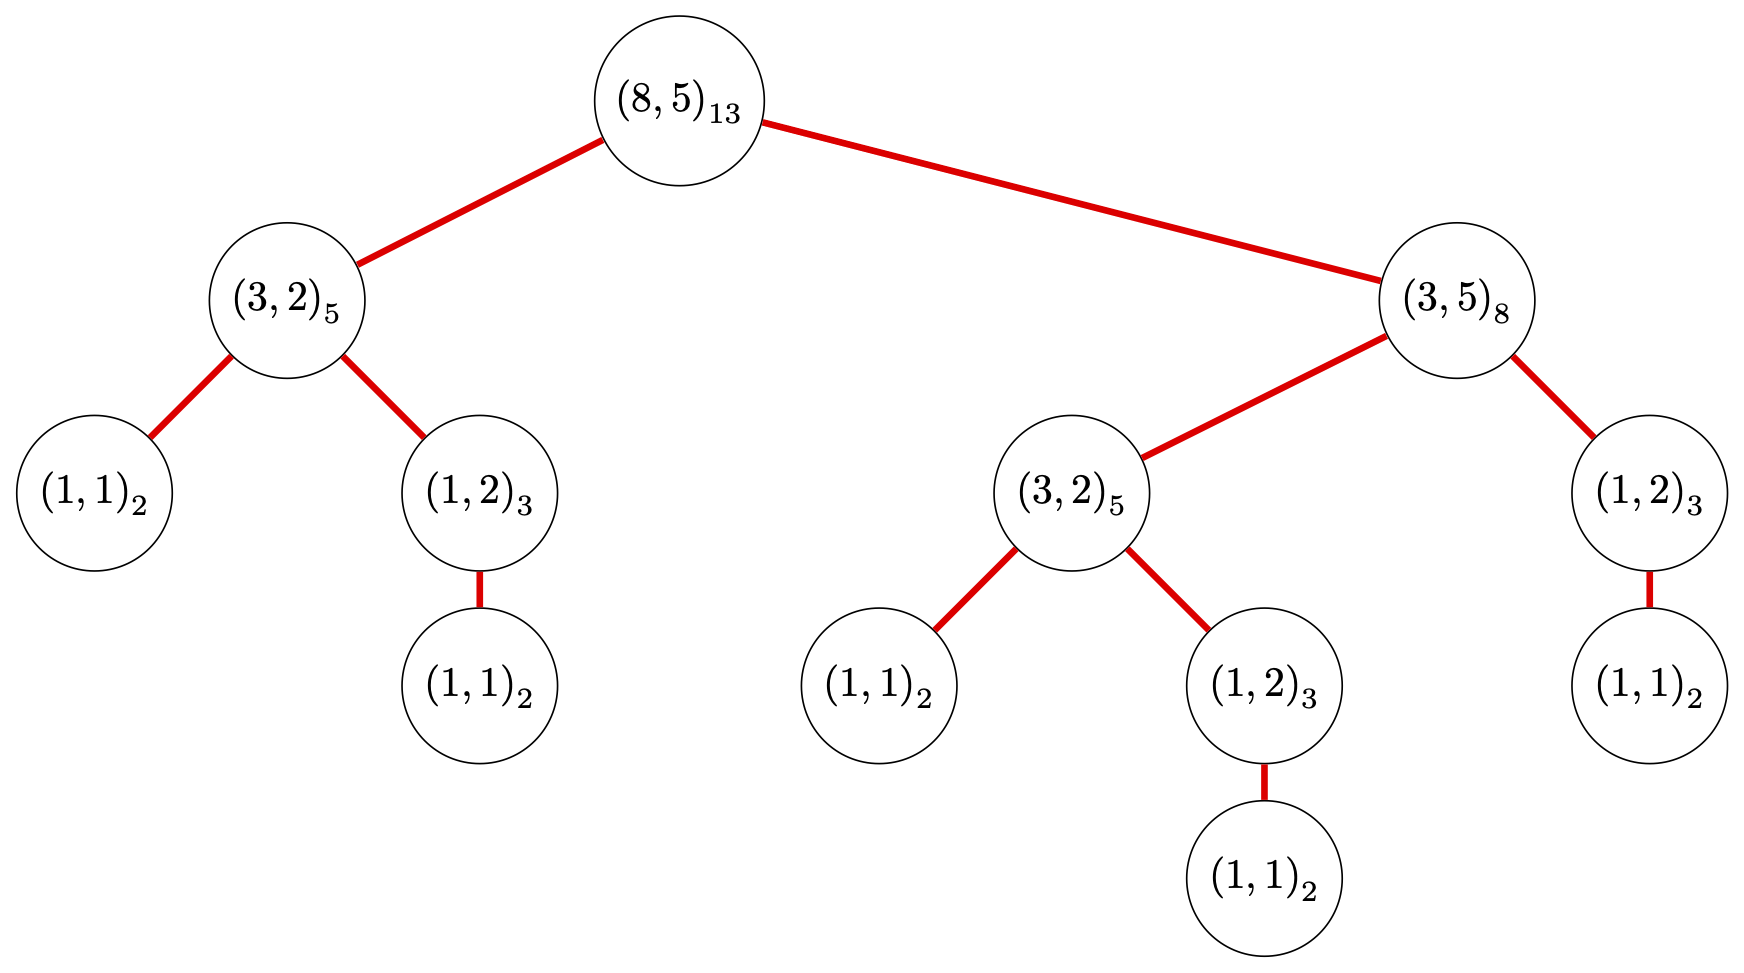
\includegraphics[width=0.8\textwidth]{fibo}
\end{figure}

\begin{proposition}
    Si $a, b \in \mathbb{Z}$, alors
    \[ {(a, b)}_n \in \JS \implies \forall k \in \mathbb{Z}^\times : {(a, b)}_{n+kab} \in \JS. \]
\end{proposition}

\begin{example}
    ${[(3, 2)]}_5 \in \JS \implies {(3, 2)}_{11} \in \JS$
\end{example}

\begin{figure}[h]
    \caption{${(3, 2)}_5 \cong {(3, 2)}_{11}$}
    \centering
    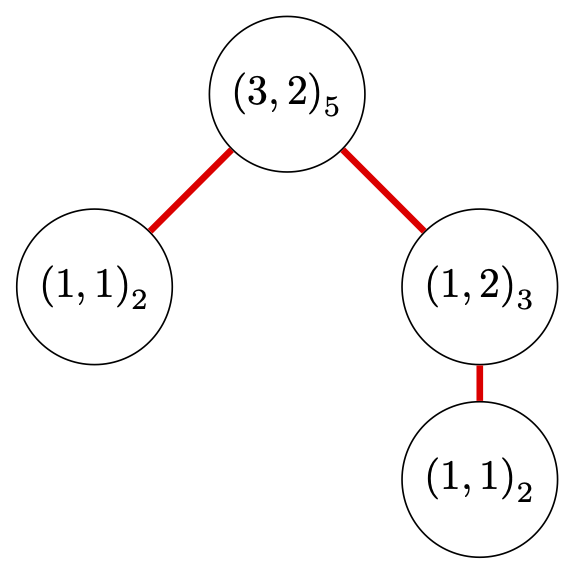
\includegraphics[width=0.3\textwidth]{532}
    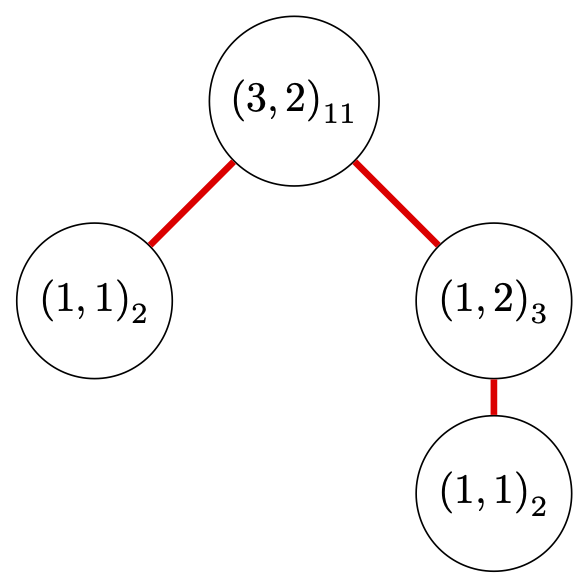
\includegraphics[width=0.3\textwidth]{11_3_2}
\end{figure}

\newpage

\section{Nouveaux résultats}

Soient $m, n \in \mathbb{N}$ tels que $m, n \geq 2$ et $[a] = {([a_1], \dots, [a_m])}_n \in S_n^m$ une singularité.

\subsection{Existence d'un éclatement}

\begin{proposition}
    Toute singularité isolée admet un éclatement.
\end{proposition}

\begin{proof}
    Prenons $(a_1, \dots, a_m) \in [a]$ le représentant naturel de $[a]$

    On cherche $(b_1, \dots, b_m) \in [a]$ tels que $\forall i \neq j : b_i \perp b_j$ et $\forall i : b_i \perp n$

    Il suffit de prendre $b_1 = a_1$ et $\forall i = 2..m$, un $b_i$ vérifiant
    \begin{align*}
        b_i & \equiv a_i \pmod n \\
        b_i & \equiv 1 \pmod {b_1} \\
            & \vdotswithin{\equiv} \\
        b_i & \equiv 1 \pmod {b_{i-1}}
    \end{align*}

    De tels $b_i$ existent par le théorème des restes chinois.

    On vérifie les coprimalités nécessaires grâce aux propriétés de $\gcd$. En effet,
    
    \hspace{\parindent} On a par la première congruence que $\forall i : b_i \perp n$ (puisque $\forall i : a_i \perp n$).

    \hspace{\parindent} Et par les suivantes $\forall i \neq j : b_i \perp b_j$.

    On a donc bien que $b = (b_1, \dots, b_m)$ est un éclatement de $[a]$.
\end{proof}

\subsection{Propriétés}

\subsubsection{Symétrie}

\begin{proposition}
    Le réarrangement des poids préserve le type $\J$. Soit $\sigma \in S_m$, on a
    \[ [a] \in \J \implies \sigma([a]) \in \J. \]
\end{proposition}

\begin{proof}
    Prenons $a \in [a]$ tel que $E_a \subset \J$. Il suffit d'observer que $E_a \cong E_{\sigma(a)}$.
\end{proof}

\begin{figure}[h]
    \caption{Illustration avec $a = (a_1, a_2)$, $\sigma = (12)$}
    \centering
    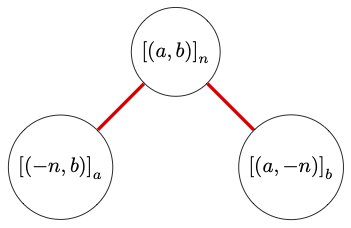
\includegraphics[width=0.4\textwidth]{abn}
    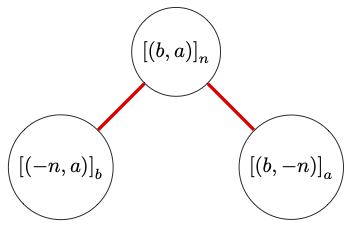
\includegraphics[width=0.4\textwidth]{ban}
\end{figure}

\subsubsection{Ajout de poids}

\begin{proposition}
    L'ajout de poids de valeur 1 préserve le type $\J$:
    \[ {([a_1], \dots, [a_m])}_n \in \J \implies {([a_1], \dots, [a_m], [1])}_n \in \J. \]
\end{proposition}

\begin{proof}
    Prenons $a \in [a]$ tel que $E_a \subset \J$, $b = (a_1, \dots, a_m, 1)$. Il suffit d'observer que $E_a \cong E_b$
\end{proof}

\begin{figure}[h]
    \caption{Illustration avec $a = (a_1, a_2)$}
    \centering
    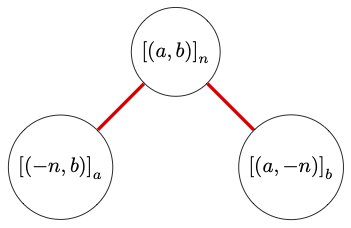
\includegraphics[width=0.4\textwidth]{abn}
    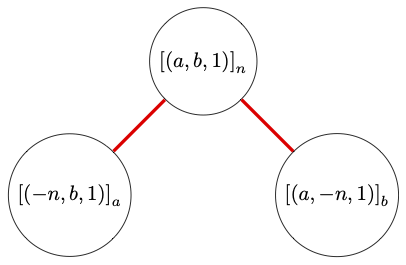
\includegraphics[width=0.4\textwidth]{ab1n}
\end{figure}

\subsubsection{Retrait de poids}

\begin{proposition}
    Le retrait de poids préserve le type $\J$:
    \begin{align*}
        {([a_1], \dots, [a_m])}_n \in \J \implies {([a_1], \dots, [a_{m-1}])}_n \in \J.
    \end{align*}
\end{proposition}

\begin{proof}
    Prenons $a \in [a]$ tel que $E_a \subset \J$.

    La preuve se fait par induction structurelle.

    D'abord, on observe ${([1], \dots, [1])}_n \in \J$.

    Puis on suppose que $\forall [b] \in E_a : [b] \in \J \implies {([b_1], \dots, [b_{m-1}])}_n \in \J$.

    On en conclut ${([a_1], \dots, [a_{m-1}])}_n \in \J$.
\end{proof}

\begin{figure}[h]
    \caption{Illustration pour $m = 3$}
    \centering
    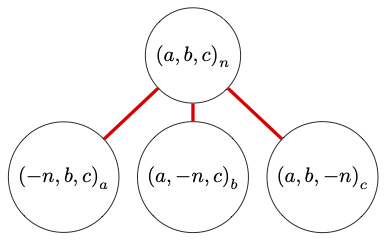
\includegraphics[width=0.4\textwidth]{abcn}
    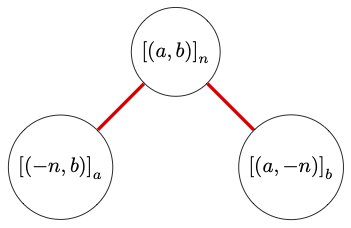
\includegraphics[width=0.4\textwidth]{abn}
\end{figure}

\newpage

\subsection{Caractérisation stricte}

\subsubsection{Frontière}

\begin{proposition}
    Soit $[a] \in S_n^2$, d'éclatement naturel $a = (a_1, a_2) \in [a]$. Alors
    \[ [a] \in \JS \implies n \geq a_1 + a_2. \]
\end{proposition} 

\begin{proof}
    Par contraposée, supposons $n < a_1 + a_2$ ($\star$)

    \begin{itemize}
        \item Si $a_1 = a_2$ ($\neq 1$ par ($\star$)), alors $[a] \not \in \JS$.
        \item Sinon, $a_1 \neq a_2$, et on peut supposer sans perdre de généralité que $a_1 > a_2$.

            Considérons $a^1$ l'éclatement naturel de $[a^1] \in E_a$ la singularité associée à $a_1$.

            On a que $a^1 = (-n \mod a_1,\; a_2 \mod a_1)$.

            Puisque $a_1 > a_2$, on a $2a_1 > a_1 + a_2 > n$, donc $a_1 < n < 2a_1$.
                
            On en déduit que $(-n \mod a_1) = 2a_1 - n$.

            Aussi, $(a_2 \mod a_1) = a_2$ car $a_1 > a_2$.

            On a donc $a^1 = (2a_1-n,\; a_2)$.

            Puisque $n < a_1 + a_2$, on a $a_1 < 2a_1 - n + a_2$.

            Donc $[a^1] \in S_{a_1}^2$ vérifie la condition ($\star$). 
            
            En répétant le raisonnement avec $[a^1]$, 
            on voit en itérant que l'arbre d'éclatements de $[n]$ 
            contient un élément $[b] \in S_a^2$ avec représentant 
            $(b_1, b_2) \in \mathbb{Z}^2$ tel que $1 < b_1 = b_2 < k$.

            Donc $[b] \not \in \JS$ et, a fortiori $[a] \not \in \JS$.
    \end{itemize}
\end{proof}

\begin{example}
    ${(4, 3)}_5 \not \in \JS$ car $5 < 4 + 3$
\end{example}

\begin{figure}[h]
    \caption{Singularités $s \in S_{32}^2$ telles que $s \in \JS$}
    \centering
    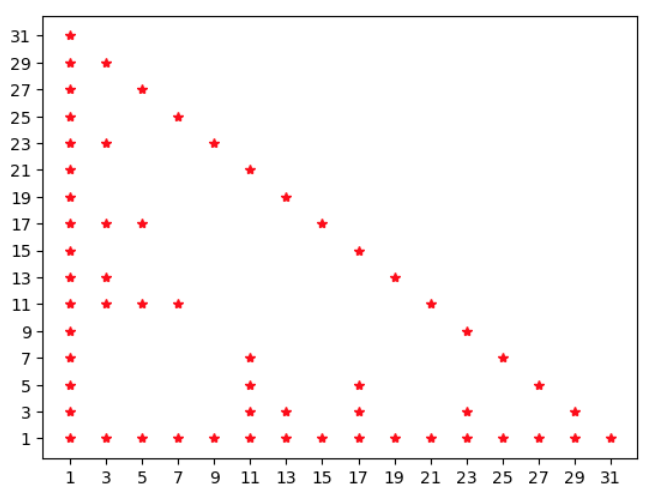
\includegraphics[width=0.6\textwidth]{singularite_j_strict_m2_n32}
\end{figure}

\newpage

\section{Conjectures}

\subsection{Combinaison linéaire}

\begin{conjecture}
    Soit ${(a, b)}_n \in \JS$, alors $\exists \alpha, \beta \in \mathbb{N}_{>0}$ tels que
    \[ \alpha a + \beta b = n \]
\end{conjecture}

Argument heuristique potentiel

Puisque $a \perp b$, prenons $s, t \in \mathbb{Z}$ tels que $1 = as + bt$ (par Bézout).

Considérons les systèmes modulaires suivants:
\begin{align*}
    x \equiv 0 \pmod a &\quad y \equiv n \pmod a, \\
    x \equiv n \pmod b &\quad y \equiv 0 \pmod b.
\end{align*}

Par le Théorème des restes chinois, l'unique solution est:
\begin{align*}
    x \equiv nas \pmod {ab} \\
    y \equiv nbt \pmod {ab}
\end{align*}

On a donc (toujours modulo $ab$)
\begin{align*}
    x + y & \equiv nas + nbt \\
            & \equiv n(as + bt) \\
            & \equiv n
\end{align*}

Et comme $a \vert x$ et $b \vert y$, prenons $\alpha = \frac{x}{a}$ et $\beta = \frac{y}{b}$, des entiers
\begin{align*}
    n & \equiv x + y \\
        & \equiv \frac{x}{a}a + \frac{y}{b}b \\
        & \equiv \alpha a + \beta b
\end{align*}

Il reste à montrer que cette égalité n'est pas seulement vraie dans $\mathbb{Z}_{ab}$ mais aussi dans $\mathbb{Z}$.

Une piste de recherche explorée jusqu'ici sans succès passe par le probème des pièces de monnaie. 
On peut reformuler la conjecture comme suit: ${(a, b)}_n \in \JS$ implique que $n$ est représentable 
par $a$ et $b$ (c'est-à-dire somme de multiples strictement positifs de $a$ et $b$) 
($\exists \alpha, \beta \in \mathbb{N}_{>0}, \alpha a + \beta b = n$), même si $n < g(a, b) = ab - (a + b)$ le nombre de Frobenius\cite[page 134]{sylvester1882}.
Il est connu que la moitié de ces nombres $a + b < n < g(a, b)$ (ceux de la forme $n = ab - ka - qb$) sont non-représentables.
Montrer que ces ${(a, b)}_n \not \in \JS$ suffirait à montrer la conjecture.

\subsection{Anti-symétrie}

\begin{corollary}
    Soit $[s] \in S_n^2$ d'éclatement naturel $(a, b) \in [s]$, avec $a, b > 1$. Alors

    \[ {(a, b)}_n \in \JS \implies {(-a, b)}_n \not \in \JS. \]
\end{corollary}

\begin{proof}
    Supposons ${(a, b)}_n \in \JS$

    La chaine d'éclatements naturels à gauche successifs de ${(-a, b)}_n$ est, pour $i > 0$, $n - ia > 0$
    \begin{align*}
        {(n - ia, b)}_{n-(i-1)a}.
    \end{align*}

    Prenons $\alpha, \beta \in \mathbb{N}_{>0}$ tels que $\alpha a + \beta b = n$ comme énoncé dans la conjecture 1.

    On a que, lorsque $i = \alpha$, $n - ia = n - \alpha a = \beta b$.

    Donc $b \vert (n - ia)$. 
    
    Puisque $b > 1$, $b \not \perp (n - ia)$, ce qui montre que ${(n - ia, b)}_n \not \in \JS$ de sorte que ${(-a, b)}_n \not \in \JS$.
\end{proof}

\newpage

\subsection{Échange racine-poids}

\begin{corollary}
    Soit $[s] \in S_n^2$ d'éclatement naturel $(a, b) \in [s]$, avec $a, b > 1$. Alors
    
    \[ {(a, b)}_n \in \JS \implies {(n, b)}_a \not \in \JS. \]
\end{corollary}

\begin{proof}
    Supposons que ${(a, b)}_n \in \JS$.

    Donc son éclatement ${(-n, b)}_a \in \JS$, de sorte que, par anti-symétrie, ${(n, b)}_a \not \in \JS$
\end{proof}

\subsection{Restriction au bord}

\begin{corollary}
    Soit $[s] \in S_n^3$ d'éclatement naturel $(a, b, c) \in [s]$, avec $a, b, c > 1$. Alors
    
    \[ {(a, b, c)}_n \not \in \JS. \]
\end{corollary}

\begin{proof}
    Si ${(a, b, c)}_n \in \JS$, alors ses éclatements ${(-n, b, c)}_a \in \JS$ et ${(a, -n, c)}_b \in \JS$

    Par retrait de poids, ${(b, c)}_a \in \JS$ et ${(a, c)}_b \in \JS$, ce qui contredit l'échange racine-poids du corollaire précédant.
\end{proof}

\begin{corollary}
    Pour être de type $\JS$, une singularité ne peut avoir plus de 2 poids supérieurs à 1.
\end{corollary}

\begin{proof}
    Si une singularité de type $\JS$ contient les poids $a, b, c > 1$, alors, par retrait de poids ${(a, b, c)}_n \in \JS$, contradiction.
\end{proof}

\begin{example}
    On observe que les singularités de type $\JS$ de $S_n^3$ sont sur le bord
\end{example}
\begin{figure}[h]
    \caption{Singularités $s \in S_{13}^3$ telles que $s \in \JS$}
    \centering
    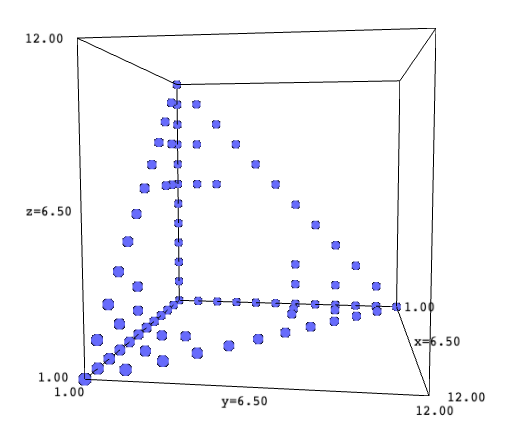
\includegraphics[width=0.7\textwidth]{singularite_j_strict_m3_n13}
\end{figure}

\begin{conjecture}
    Si $[a] \in \JS$, alors $[a] \in \J$, donc $\J = \JS$
\end{conjecture}

\bibliographystyle{plain} % We choose the "plain" reference style
\bibliography{refs} % Entries are in the refs.bib file

\end{document}